\begin{frame}\begin{center}
\LARGE\textbf{Computational Model}
\end{center}\end{frame}
%-------------------------------------------------------------------------------
%-------------------------------------------------------------------------------
\begin{frame}
\textbf{Additional Structure}
\begin{align*}\begin{array}{ll}
t & \text{age} \\
k       & \text{unobserved type} \\
x_{j,t} & \text{experience in occupation $j$ at age $t$} \\
a_t     & \text{action at age $j$} \\
g_t     & \text{level of schooling at age $t$}
\end{array}\end{align*}
\end{frame}
%-------------------------------------------------------------------------------
%-------------------------------------------------------------------------------
\begin{frame}

\textbf{Skill Production Function}

\begin{align*}
e_{j,k,t} & =  \exp\{ e_{j,k,16}+ \underbrace{\alpha_{j,1} g_t + \alpha_{j,2} \Ind[g_t \geq 12] + \alpha_{j,3} \Ind[g_t \geq 16]}_{\text{schooling}}\\
                & + \underbrace{\alpha_{j,4} x_{j,t} + \alpha_{j,5} x^2_{j, t} + \alpha_{j,6} \Ind[x_{j, t} > 0] + \alpha_{j,7} x_{j\neq j^\prime, t}}_{\text{work experience}}  \\
                & + \underbrace{\alpha_{j,8}\Ind[a_{t - 1} \neq j] }_{\text{depreciation}} + \alpha_{j,9} (t - 16) + \alpha_{j,10} \Ind[t < 18] + \epsilon_{j, t}\}
\end{align*}

with $j, j^\prime = 1, 2$, $k = 1, \hdots,4$, and $t=16,\hdots,65$

\end{frame}
%-------------------------------------------------------------------------------
%-------------------------------------------------------------------------------
\begin{frame}

\textbf{Labor Market}

\begin{align*}
r_{j,k,t} & =   w_{j,k,t} + \underbrace{\kappa_{1}\Ind[g_t \geq 12] + \kappa_{2} \Ind[g_t \geq 16]}_{\text{common returns}} + \beta_{j,1} \\
          & + \underbrace{\beta_{j,2}\Ind[x_{j,t} > 0, a_{t-1}\neq j] + \beta_{j,3}\Ind[x_{j, t} = 0, a_{t-1}\neq j ]}_{\text{entry cost}}
\end{align*}

with $w_{j,k, t} = r_j e_{j,k,t}$
\end{frame}
%-------------------------------------------------------------------------------
%-------------------------------------------------------------------------------
\begin{frame}

\textbf{School}
\begin{align*}
r_{3,k,t} & = e_{3,k,16} + \underbrace{\gamma_{1}\Ind[g_t \geq 12] + \gamma_{2} \Ind[g_t \geq 16]}_{\text{monetary and psychic cost}} \\
         & + \underbrace{\gamma_{3} \Ind[a_{t -1} \neq 3, g_t \leq 11]  + \gamma_{4} \Ind[a_{t -1} \neq 3, g_t \geq 12]}_{\text{reenrollment cost}}  \\
         & + \gamma_{5} (t - 16) + \gamma_{6} \Ind[t \le 18] + \underbrace{\kappa_{1}\Ind[g_t \geq 12] + \kappa_{2} \Ind[g_t \geq 16]}_{\text{common returns}} \\
         & + \epsilon_{3,t}
\end{align*}
\end{frame}

%-------------------------------------------------------------------------------
%-------------------------------------------------------------------------------
\begin{frame}
\textbf{Home}
\begin{align*}
r_{4,k,t} & = e_{4,k,16} + \zeta_{1} \Ind[18 \leq t \leq 20] +  \zeta_{2} \Ind[t \geq 21] \\
          & + \underbrace{\kappa_{1}\Ind[g_t \geq 12] + \kappa_{2} \Ind[g_t \geq 16]}_{\text{common returns}} + \epsilon_{4,t}
\end{align*}
\end{frame}
%-------------------------------------------------------------------------------
%-------------------------------------------------------------------------------
\begin{frame}
\textbf{State Space}\vspace{0.3cm}
\begin{itemize}
\item at time $t$
\begin{align*}
s_t  = & \{g_t,  \{x_{j, t}\}_{j=1,2}, a_{t-1}, \{\epsilon_{j, t}\}_{j=1,\hdots,4}\}\\
\bar{s}_t  = & \{g_t,  \{x_{j, t}\}_{j=1,2}, a_{t-1}\}
\end{align*}
\item laws of motion
\begin{align*}
x_{j,t + 1} & = x_{j,t} + \Ind[a_t = j]  \qquad\forall\quad j \in \{1, 2\}  \\[1em]
g_{t + 1}    & = g_t + \Ind[a_t = 3]
\end{align*}
\end{itemize}
\end{frame}
%-------------------------------------------------------------------------------
%-------------------------------------------------------------------------------
\begin{frame}

\textbf{Distribution of shocks}
\begin{align*}
[\epsilon_{1,t}, \epsilon_{2,t}, \epsilon_{3,t}, \epsilon_{4,t}]^T \sim \mathcal{N}_0(\vec{0}, \Sigma)\\
\end{align*}

\end{frame}
%-------------------------------------------------------------------------------
%-------------------------------------------------------------------------------
\begin{frame}
\begin{figure}\caption{Value Functions}
\scalebox{0.35}{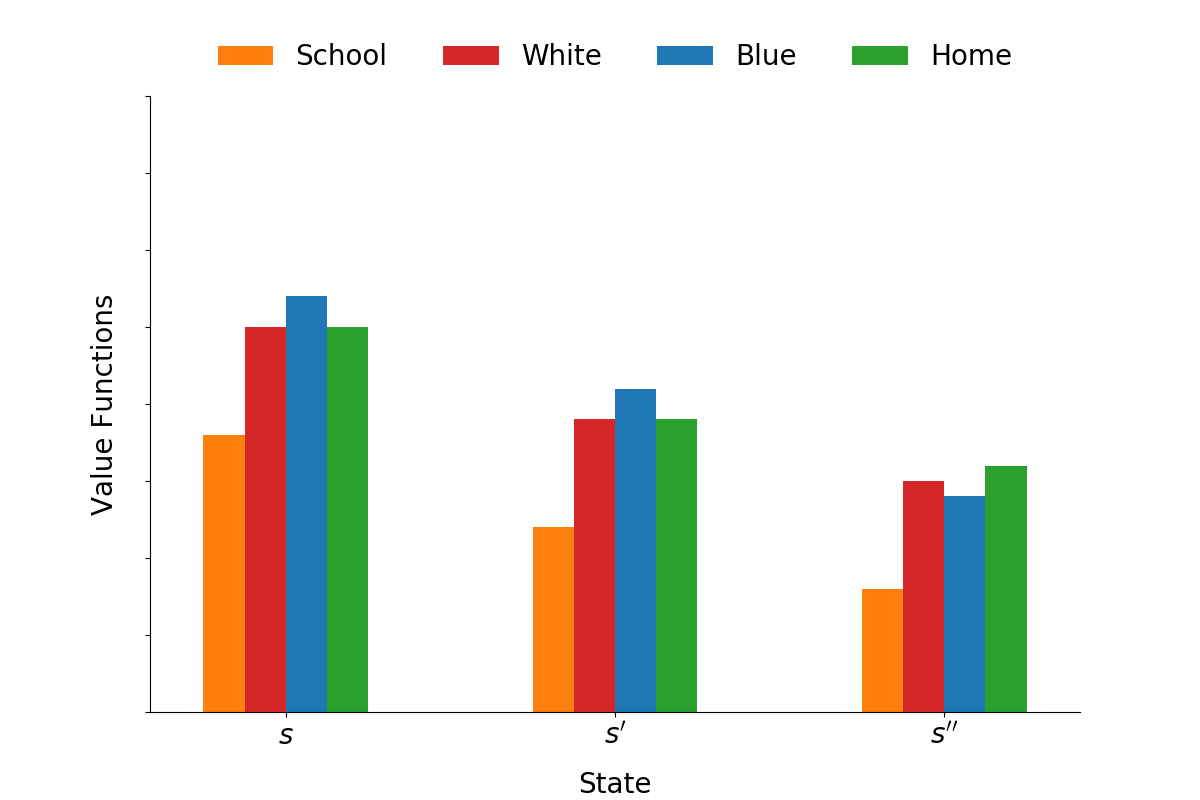
\includegraphics{fig-admissible-values}}
\end{figure}
\end{frame}
%-------------------------------------------------------------------------------
%-------------------------------------------------------------------------------
\begin{frame}

\textbf{Computational Tool}

\begin{center}
\url{https://respy.readthedocs.io}
\end{center}

\begin{itemize}\setlength\itemsep{1em}
\item Technical Documentation\medskip
\begin{itemize}\setlength\itemsep{1em}
\item Numerical Methods, Source Codes, Test Suite
\end{itemize}
\item User Documentation\medskip
\begin{itemize}\setlength\itemsep{1em}
\item Tutorial
\end{itemize}
\end{itemize}\medskip
$\Rightarrow$ Transparency, Recomputability, and Extensibility
\end{frame}
%-------------------------------------------------------------------------------
%-------------------------------------------------------------------------------
